\documentclass{beamer}
\usepackage{graphicx}
\usepackage{paralist}
\usepackage{outlines}

\title{How to Organize Your Projects}
\author{Mendocino College - DAM 110}
\titlegraphic{\vspace{-10mm}
\includegraphics[width = .8\textwidth]{images/photoshop.jpg}} 
\date{\vspace{-5em}} 


\mode <presentation>
\usetheme{Warsaw}
\usecolortheme{default}

\setbeamerfont{footline}{size=\fontsize{5}{8}\selectfont}

\definecolor{darkred}{rgb}{20,0,0}
\definecolor{darkgreen}{RGB}{40,110,20}
\definecolor{darkpurple}{RGB}{30,0,30}
\definecolor{chardonnay}{RGB}{255, 255, 204}

\setbeamercolor*{palette primary}{fg=white, bg=darkgreen}


\begin{document}
	{
		\setbeamertemplate{footline}{} 
		\setbeamertemplate{headline}{} 
		\begin{frame}
			\vspace{-35pt}
			\maketitle
		\end{frame}
	}

	\section{Organizing your Projects}
		\begin{frame}
		\frametitle{Filters}
		\begin{center}
			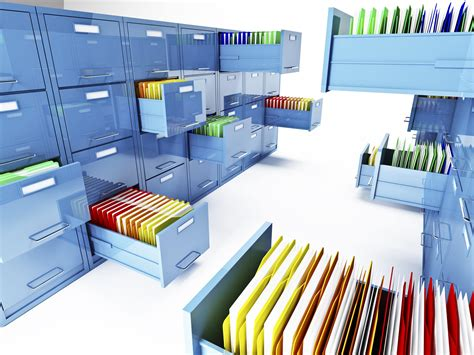
\includegraphics[width = 0.8\textwidth]{images/th (1).jpg}
		\end{center}
	\end{frame}
	
			\subsection{Windows File Explorer}		
	\begin{frame}
		\frametitle{Windows File Explorer}
\begin{center}
	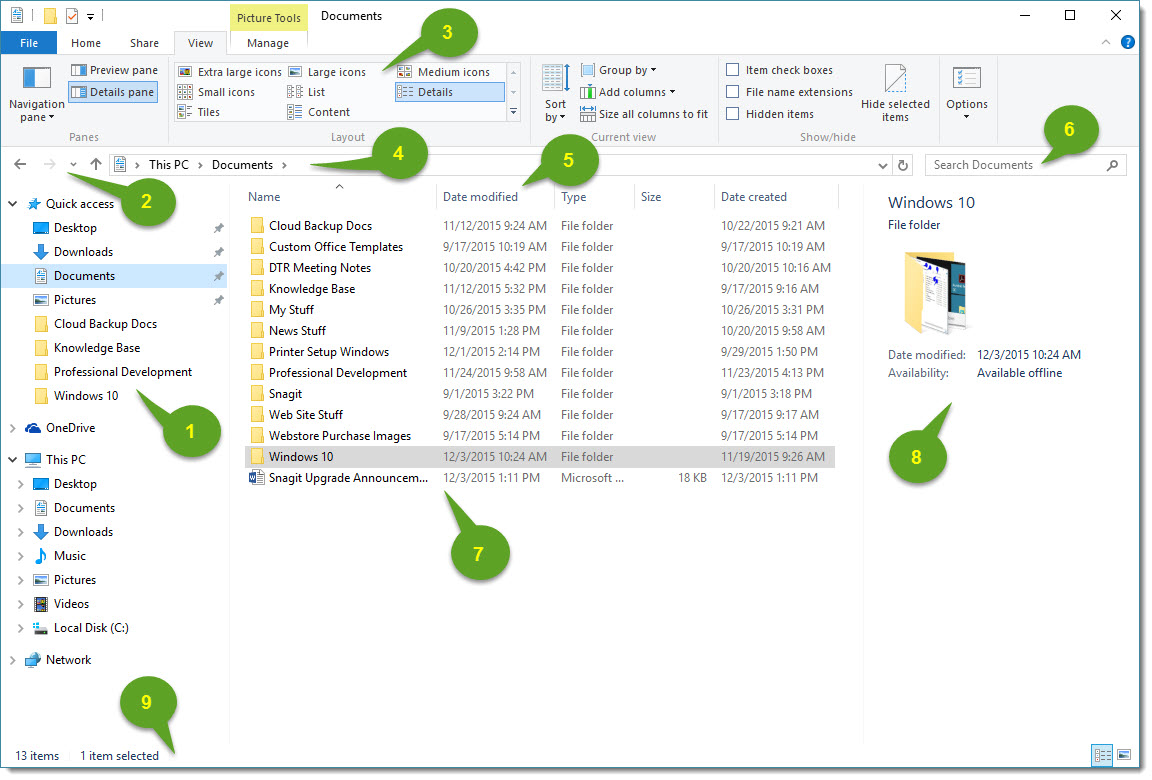
\includegraphics[width=.7\textwidth]{images/win10-fileexplorer-overview-callouts_0.jpg}
	\end{center}
		\end{frame}
	
\begin{frame}
	\frametitle{How to Make a new Folder}
	
	\begin{outline}
		\1 Right-Click anywhere within the main area of the Windows Explorer.  
		\2 Hover over New
		\3 Left-Click "Folder"
	\end{outline}
	\begin{center}
		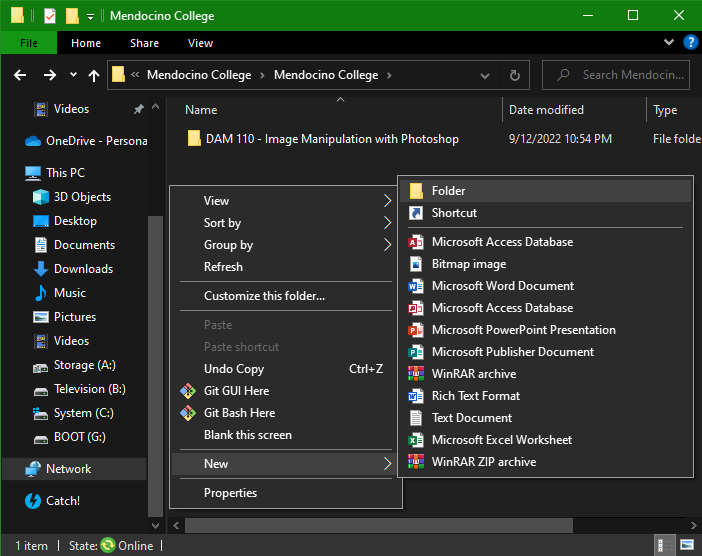
\includegraphics[width=.7\textwidth]{images/new folder.png}
	\end{center}
\end{frame}

\subsection{Class Folder Structure}	
\begin{frame}
		\frametitle{Class Folder Structure}

	\begin{outline}
		\1 Documents
		\2 Mendocino College
		\3 DAM 110 - Image Manipulation with Photoshop
		\3 Separate by each week, Assignments and Projects.
	\end{outline}
\begin{center}
	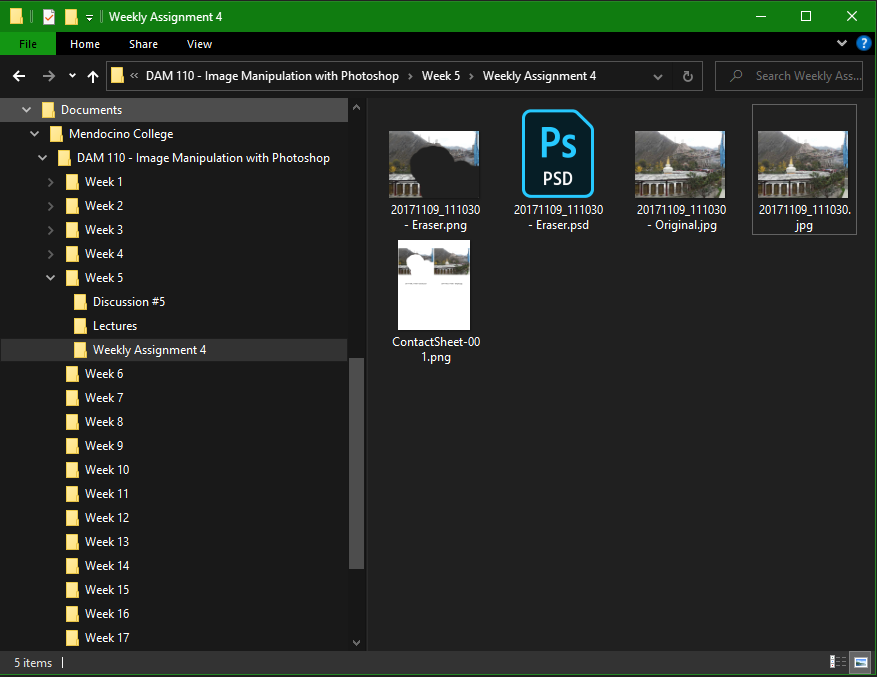
\includegraphics[width=.7\textwidth]{images/Class Folder Structure.png}
	\end{center}
\end{frame}

	\section{Backing Up Your Work on Google Drive}	
		\begin{frame}
		\frametitle{Google Drive}
		\begin{center}
			
\includegraphics[width = 1.0\textwidth]{images/Download-Google-Drive-for-Windows.png}
		\end{center}
	\end{frame}
	
	\subsection{Access your Mendocino College Google Drive}
	\begin{frame}
		\frametitle{How to Access your Mendocino College Google Drive - Step 1}
	\begin{outline}
	\1 Sign into MyMendocino at:
	\1 https://my.mendocino.edu/
\end{outline}
	\end{frame}

	\begin{frame}
	\frametitle{How to Access your Mendocino College Google Drive - Step 2}
	\begin{outline}
	\1 Go to your google drive at:
	\1 https://drive.google.com/drive/u/7/my-drive
\end{outline}
\end{frame}

	\subsection{Save Your Files to Google Drive}
\begin{frame}
	\frametitle{Saving your Files to Google Drive}
	\begin{outline}
		\1 Drag your class folder into Google Drive
	\end{outline}
		\begin{center}
	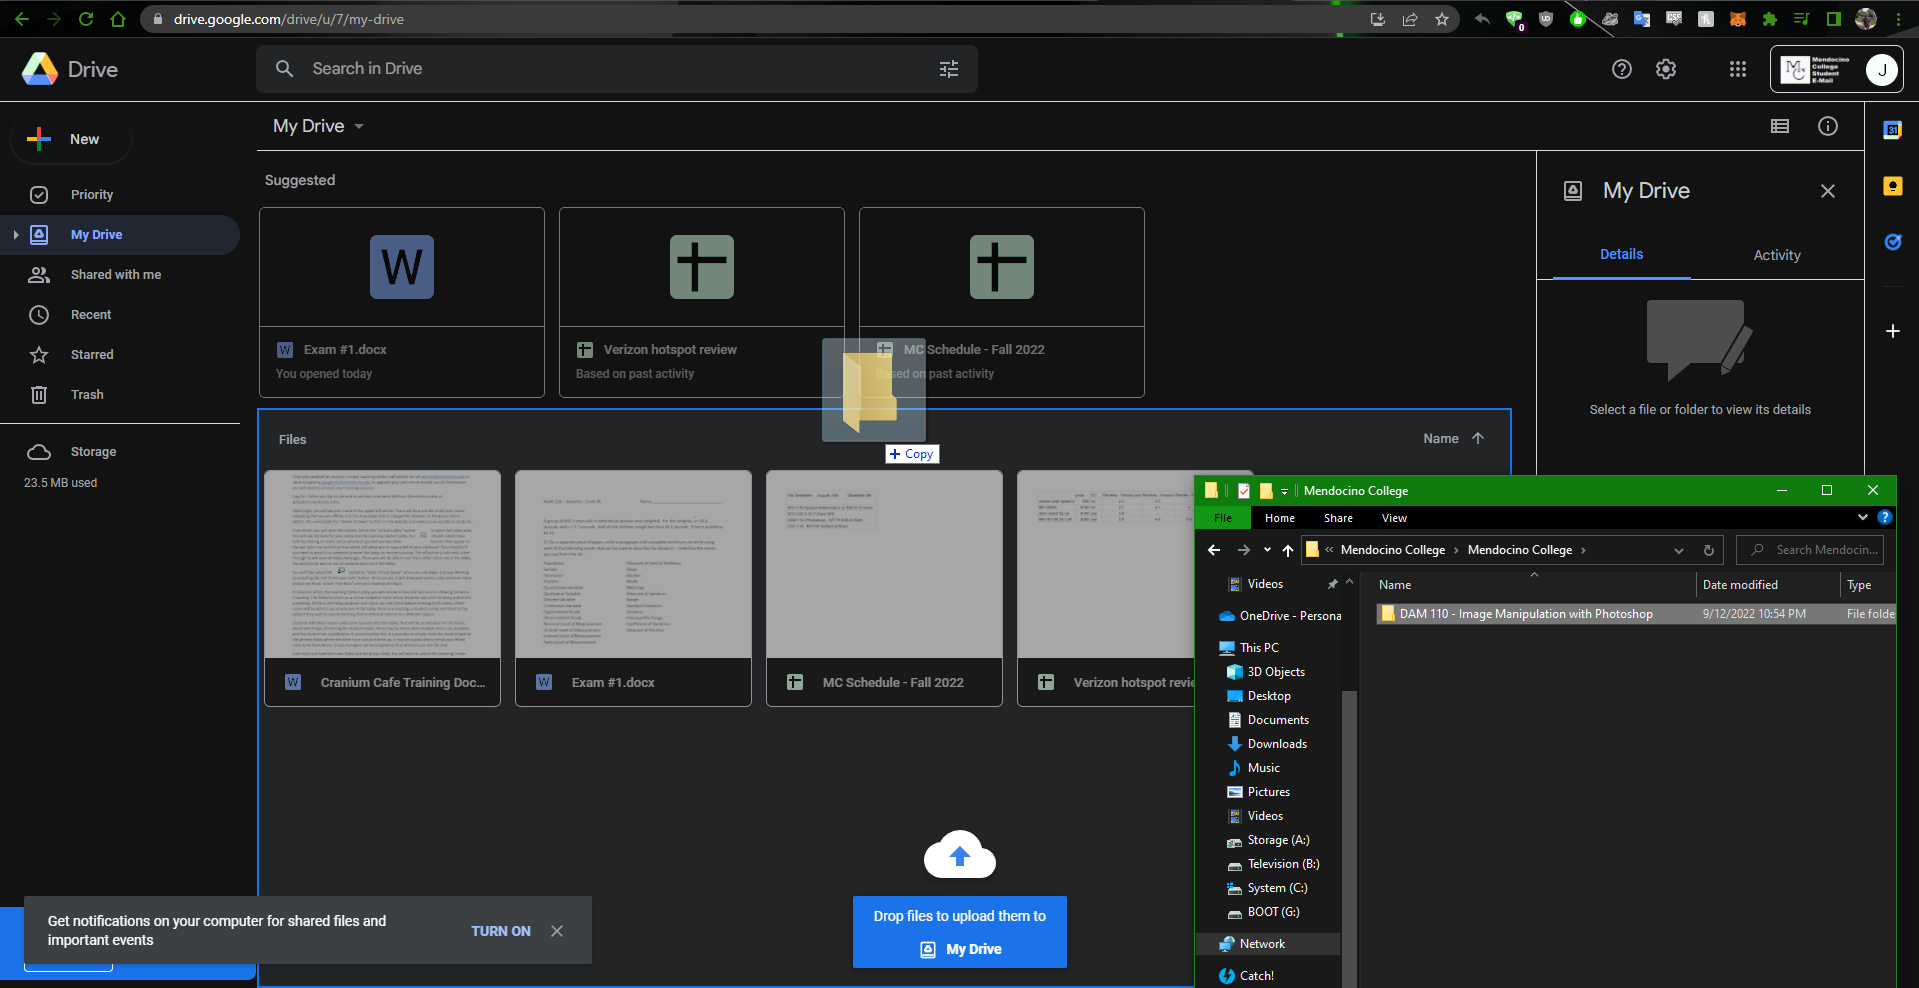
\includegraphics[width = 1.0\textwidth]{images/backing up with google drive.png}
\end{center}
\end{frame}


\end{document}